

\section{Problem 3}
\label{part3}
\begin{verbatim}
3. Re-download the 1000 TimeMaps from A2, Q2.  Create a graph where
the x-axis represents the 1000 TimeMaps.  If a TimeMap has ``shrunk'',
it will have a negative value below the x-axis corresponding to the
size difference between the two TimeMaps.  If it has stayed the
same, it will have a ``0'' value.  If it has grown, the value will be 
positive and correspond to the increase in size between the two
TimeMaps.

As always, upload all the TimeMap data.  If the A2 github has the 
original TimeMaps, then you can just point to where they are in 
the report.


\end{verbatim}

\subsection{Solution}
\begin{enumerate}
\item For this question I need to get data from my Assignment 2.
\item I have taken the code from the assignment 2 and executed it again which gives me a complete different set of TimeMaps. So, Now I have old and new TimeMaps which should be used to get solution for this question.
\item Python code for getting the new TimeMaps can be found in listing\ref{lst:q2-1}.
\item The input I gave to the above code can be found in fig\ref{Sampleti1}.
\item So, Now I subtracted the old TimeMaps from the New TimeMaps which gives me the difference between both of them.
\item This difference in the TimeMaps is then plotted using the following R code which can be seen in listing\ref{lst:q2-2}.
\item The plotted graph can be seen in the fig\ref{Samplet1}.
\item So by this we can know that there have been positive increase and negative increase from new and old TimeMaps data.
\end{enumerate}
\newpage

\subsection{Code Listing 1}

\lstinputlisting[language=Python,breaklines = true,frame=single,caption={Python Code for counting the number of mementos for each URI}, label=lst:q2-1,captionpos=b,numbers=left,showspaces=false,showstringspaces=false,basicstyle=\footnotesize]{get_memento_count.py}
\newpage

\subsection{Code Listing 2}

\lstinputlisting[language=R,breaklines = true,frame=single,caption={R Code for for plotting graph}, label=lst:q2-2,captionpos=b,numbers=left,showspaces=false,showstringspaces=false,basicstyle=\footnotesize]{R_code.R}
\newpage

\subsection{Input}
\begin{figure}[ht]    
    \begin{center}
        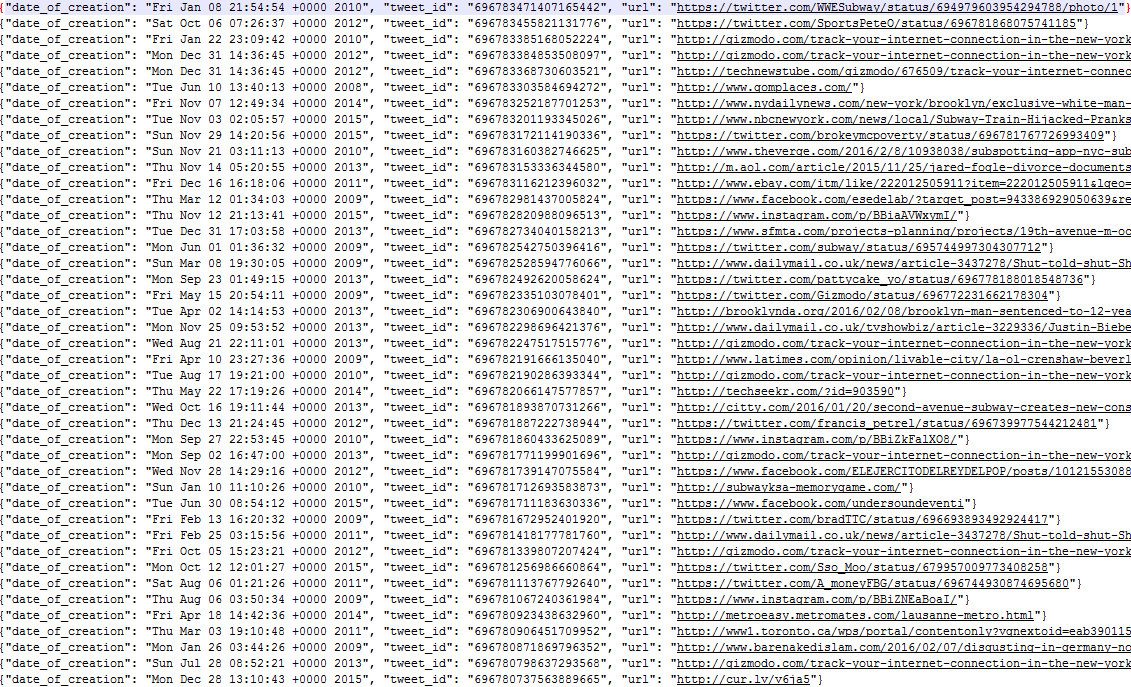
\includegraphics[scale=0.6]{sampleinput3.png}
        \caption{Sample Json data}
        \label{Sampleti1}
    \end{center}
\end{figure}
\newpage


\subsection{Outputs}
\subsubsection{Output 1}
\begin{figure}[ht]    
    \begin{center}
        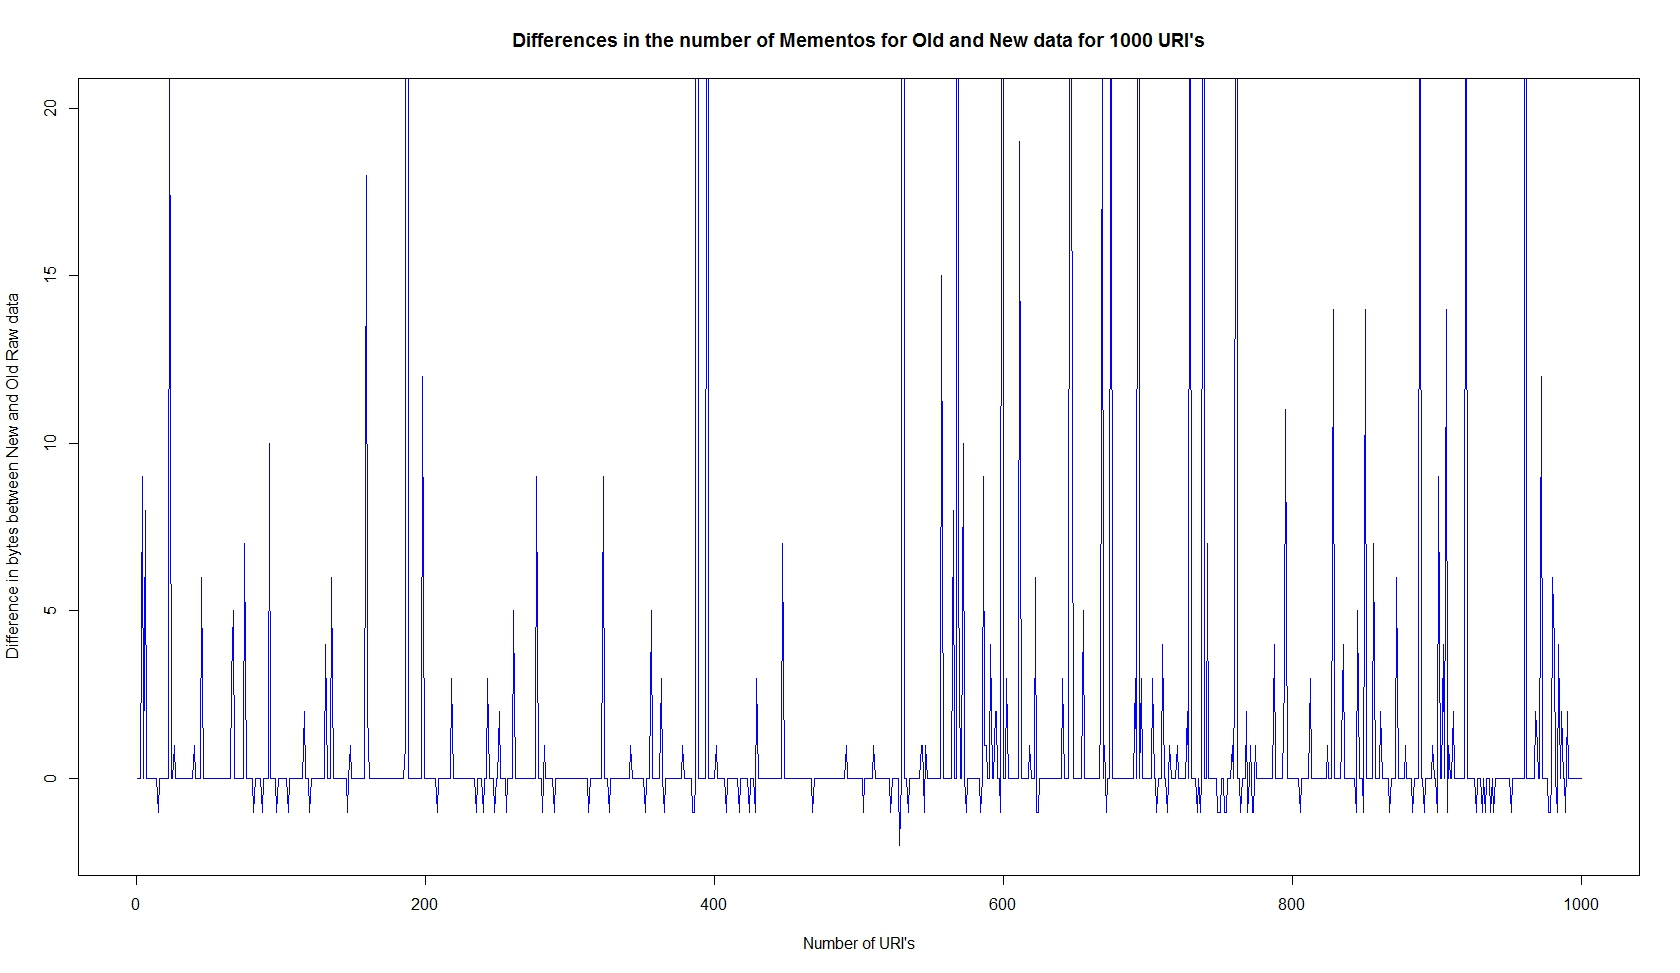
\includegraphics[scale=0.3]{differnce_graph.jpeg}
        \caption{Line graph showing differences in the number of Mementos for Old and New data for 1000 URI's }
        \label{Samplet1}
    \end{center}
\end{figure}
\newpage


